% Copyright 2004 by Till Tantau <tantau@users.sourceforge.net>.
%
% In principle, this file can be redistributed and/or modified under
% the terms of the GNU Public License, version 2.
%
% However, this file is supposed to be a template to be modified
% for your own needs. For this reason, if you use this file as a
% template and not specifically distribute it as part of a another
% package/program, I grant the extra permission to freely copy and
% modify this file as you see fit and even to delete this copyright
% notice.

\documentclass{beamer}
\usepackage[utf8]{inputenc}
\usepackage{amsmath}
\usepackage{amsthm}
\usepackage{amssymb}
\usepackage{xcolor}
\usepackage{enumerate}
\usepackage[overload]{empheq}
\usepackage{filecontents}
\usepackage{graphics}

\usepackage{graphicx}

\usetheme{Singapore}
\setbeamertemplate{navigation symbols}{}
\setbeamertemplate{footline}[frame number]{}

\title{ACO for SSCFLP}

\author{Dorian Dumez \& Samuel Buchet}

\date{may 30 2017}

\AtBeginSection[]
{
  \begin{frame}<beamer>{Contents}
    \tableofcontents[currentsection]
  \end{frame}
}
%\AtBeginSubsection[]
%{
%  \begin{frame}<beamer>{Sommaire}
%    \tableofcontents[currentsection,currentsubsection]
%  \end{frame}
%}

% Let's get started
\begin{document}

\begin{frame}
  \titlepage
\end{frame}

\begin{frame}{Table Of Content}
  \tableofcontents
  % You might wish to add the option [pausesections]
\end{frame}

\section{Single Source Capacitated Facility Location Problem}

\begin{frame}{Presentation of the problem}

    \begin{figure}
        \centering
        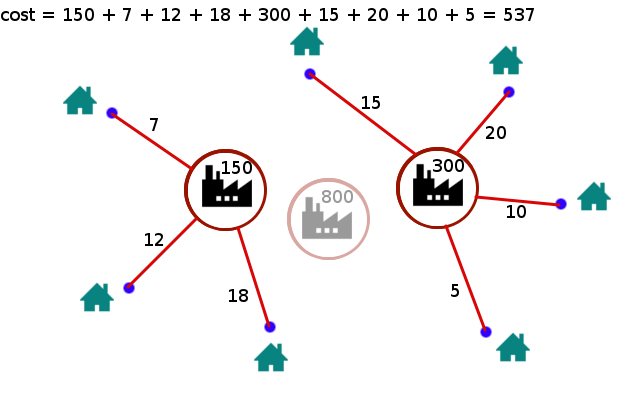
\includegraphics[scale=0.3]{schema}
    \end{figure}

    \begin{itemize}
        \item NP-hard combinatorial optimization problem
        \item m places to (eventually) open facilities
        \item n customers to be connected to the facilities
        \item each facility has an opening cost and a demand
        \item each customer has a connection cost and a capacity
        \item goal: minimize the cost
    \end{itemize}

\end{frame}

\begin{frame}{Linear program}
    \begin{figure}
    \centering
    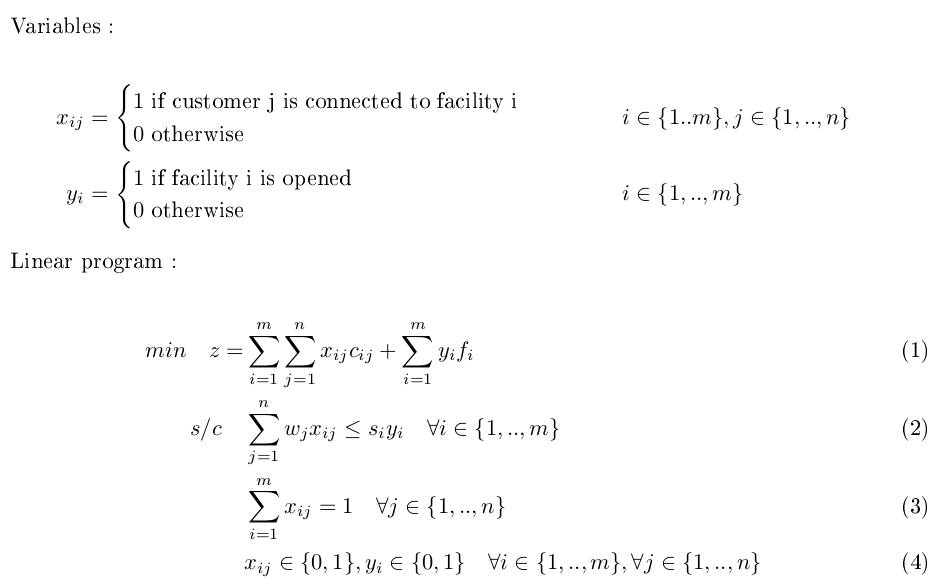
\includegraphics[scale=0.32]{model}
\end{figure}
\end{frame}

\section{Ant Colony Optimization}

\begin{frame}{Global shape}
Decisions based only on customer/facility associations:
\begin{itemize}
\item
pheromone and heuristic information are in matrices $\mathbb{R}^{n \times m}$, one value for each association
\item
heuristic information is $1/ \text{association cost}$, it does not take into account the opening cost
\item
to construct a solution we take each customer and, with the help of a roulette, we associate them with a facility with enough remaining capacity
\end{itemize}
\end{frame}

\begin{frame}{Update pheromone method}
3 designs implemented :
\begin{itemize}
\item
ACS : all ants are equal \\
$\Delta \tau_{ij} = \sum \limits_{bs \in T} \Delta \tau_{ij}^{bs}$
\item
EAS : only the best one drops off pheromone \\
$\Delta \tau_{ij} = \sum \limits_{i = 1}^{\text{nbElite}} \Delta \tau_{ij}^{bs\left[i\right]}$
\item
rank based : best one leaves behind more pheromones \\
$\Delta \tau_{ij} = \sum \limits_{i = 1}^{\text{nbAnt}} \Delta \rho^i \tau_{ij}^{bs\left[ i \right] }$, $\rho \in \left[ 0 ; 1 \right] $
\end{itemize}
Where $\Delta \tau_{ij}^{bs} = \frac{\delta_{bs.association}(i,j)}{bs.val}$
\end{frame}

\section{Local search}

\begin{frame}{Principle}
    \begin{itemize}
        \item definition of a neighborhood
        \item the neighborhood is explored
        \item hopefully a better solution is found
        \item the process is repeated until the solution cannot be improved anymore
    \end{itemize}
\end{frame}

\begin{frame}{Local Search for FLP}
    \begin{figure}
        \centering
        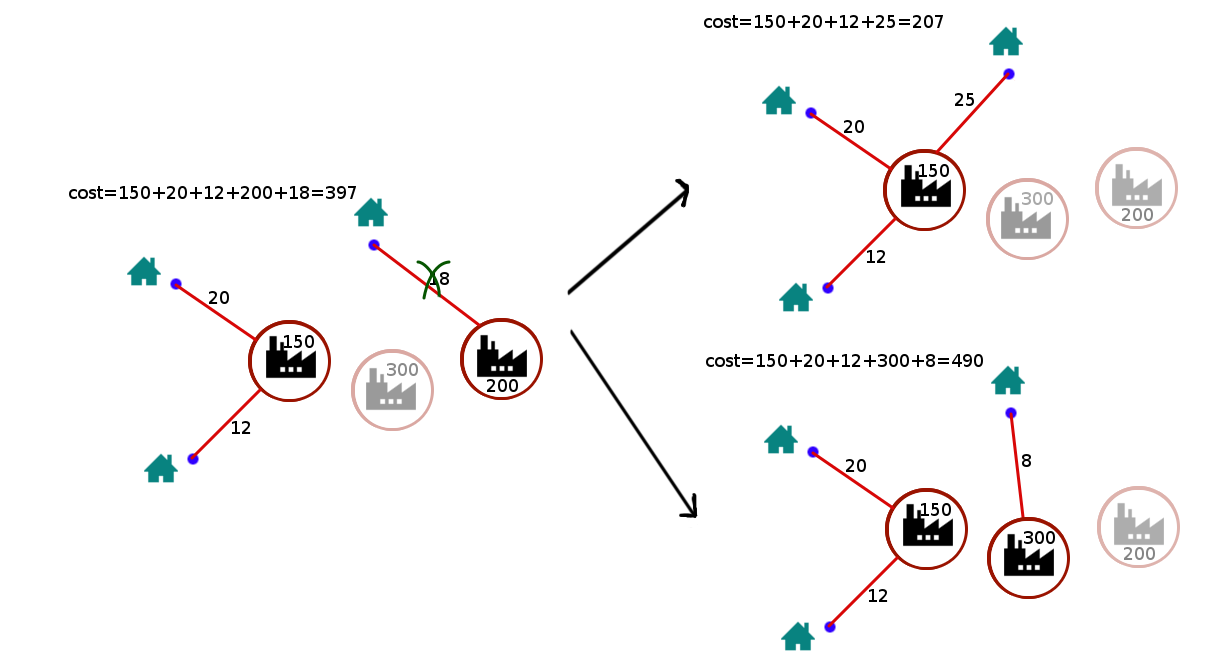
\includegraphics[scale=0.27]{schemalstot}
        \caption{ one move = connect a customer to another facility}
    \end{figure}
\end{frame}

\section{Experiments}

\begin{frame}{Using irace}
\begin{itemize}
\item
Parameter settings have already been done by irace
\item
We use a set of 71 instances of different sizes :
\begin{itemize}
\item
56 were used as training sets
\item
21 were used as testing sets
\end{itemize}
\item
At the end of the run irace concludes that it is possible to obtain better results with more time
\item<2->
Demonstration with output parameter
\end{itemize}
\end{frame}

\begin{frame}{Further improvement}
\begin{itemize}
\item
Perform a longer irace run
\item
Decide which facility to open:
\begin{itemize}
\item
modify pheromone and heuristic information
\item
adapt the construction algorithm
\end{itemize}
\item
Try other local searches, like VND
\item
Try other pheromone update schemas

\end{itemize}
\end{frame}

\section*{Conclusion}

\begin{frame}{Conclusion}
\begin{itemize}
\item
In conlcusion, we can say that the results from this research are not satisfactory, but then again, the problem is complicated.
\item
With an improved version we should be able to speed up exact algorithms
\end{itemize}
\end{frame}

\section{References}

\begin{frame}{References}

\begin{itemize}

    \item Icons made by \href{http://www.freepik.com}{Freepik} from \href{http://www.flaticon.com}{www.flaticon.com} is licensed by \href{http://creativecommons.org/licenses/by/3.0/}{Creative Commons BY 3.0}

    \item Icons made by \href{http://www.flaticon.com/authors/icomoon}{Icomoon} from \href{http://www.flaticon.com}{www.flaticon.com} is licensed by \href{http://creativecommons.org/licenses/by/3.0/}{Creative Commons BY 3.0}

\end{itemize}

\end{frame}

\end{document}
